% Options for packages loaded elsewhere
\PassOptionsToPackage{unicode}{hyperref}
\PassOptionsToPackage{hyphens}{url}
%
\documentclass[
]{article}
\usepackage{lmodern}
\usepackage{amssymb,amsmath}
\usepackage{ifxetex,ifluatex}
\ifnum 0\ifxetex 1\fi\ifluatex 1\fi=0 % if pdftex
  \usepackage[T1]{fontenc}
  \usepackage[utf8]{inputenc}
  \usepackage{textcomp} % provide euro and other symbols
\else % if luatex or xetex
  \usepackage{unicode-math}
  \defaultfontfeatures{Scale=MatchLowercase}
  \defaultfontfeatures[\rmfamily]{Ligatures=TeX,Scale=1}
\fi
% Use upquote if available, for straight quotes in verbatim environments
\IfFileExists{upquote.sty}{\usepackage{upquote}}{}
\IfFileExists{microtype.sty}{% use microtype if available
  \usepackage[]{microtype}
  \UseMicrotypeSet[protrusion]{basicmath} % disable protrusion for tt fonts
}{}
\makeatletter
\@ifundefined{KOMAClassName}{% if non-KOMA class
  \IfFileExists{parskip.sty}{%
    \usepackage{parskip}
  }{% else
    \setlength{\parindent}{0pt}
    \setlength{\parskip}{6pt plus 2pt minus 1pt}}
}{% if KOMA class
  \KOMAoptions{parskip=half}}
\makeatother
\usepackage{xcolor}
\IfFileExists{xurl.sty}{\usepackage{xurl}}{} % add URL line breaks if available
\IfFileExists{bookmark.sty}{\usepackage{bookmark}}{\usepackage{hyperref}}
\hypersetup{
  pdftitle={DSII HW1},
  hidelinks,
  pdfcreator={LaTeX via pandoc}}
\urlstyle{same} % disable monospaced font for URLs
\usepackage[margin=1in]{geometry}
\usepackage{color}
\usepackage{fancyvrb}
\newcommand{\VerbBar}{|}
\newcommand{\VERB}{\Verb[commandchars=\\\{\}]}
\DefineVerbatimEnvironment{Highlighting}{Verbatim}{commandchars=\\\{\}}
% Add ',fontsize=\small' for more characters per line
\usepackage{framed}
\definecolor{shadecolor}{RGB}{248,248,248}
\newenvironment{Shaded}{\begin{snugshade}}{\end{snugshade}}
\newcommand{\AlertTok}[1]{\textcolor[rgb]{0.94,0.16,0.16}{#1}}
\newcommand{\AnnotationTok}[1]{\textcolor[rgb]{0.56,0.35,0.01}{\textbf{\textit{#1}}}}
\newcommand{\AttributeTok}[1]{\textcolor[rgb]{0.77,0.63,0.00}{#1}}
\newcommand{\BaseNTok}[1]{\textcolor[rgb]{0.00,0.00,0.81}{#1}}
\newcommand{\BuiltInTok}[1]{#1}
\newcommand{\CharTok}[1]{\textcolor[rgb]{0.31,0.60,0.02}{#1}}
\newcommand{\CommentTok}[1]{\textcolor[rgb]{0.56,0.35,0.01}{\textit{#1}}}
\newcommand{\CommentVarTok}[1]{\textcolor[rgb]{0.56,0.35,0.01}{\textbf{\textit{#1}}}}
\newcommand{\ConstantTok}[1]{\textcolor[rgb]{0.00,0.00,0.00}{#1}}
\newcommand{\ControlFlowTok}[1]{\textcolor[rgb]{0.13,0.29,0.53}{\textbf{#1}}}
\newcommand{\DataTypeTok}[1]{\textcolor[rgb]{0.13,0.29,0.53}{#1}}
\newcommand{\DecValTok}[1]{\textcolor[rgb]{0.00,0.00,0.81}{#1}}
\newcommand{\DocumentationTok}[1]{\textcolor[rgb]{0.56,0.35,0.01}{\textbf{\textit{#1}}}}
\newcommand{\ErrorTok}[1]{\textcolor[rgb]{0.64,0.00,0.00}{\textbf{#1}}}
\newcommand{\ExtensionTok}[1]{#1}
\newcommand{\FloatTok}[1]{\textcolor[rgb]{0.00,0.00,0.81}{#1}}
\newcommand{\FunctionTok}[1]{\textcolor[rgb]{0.00,0.00,0.00}{#1}}
\newcommand{\ImportTok}[1]{#1}
\newcommand{\InformationTok}[1]{\textcolor[rgb]{0.56,0.35,0.01}{\textbf{\textit{#1}}}}
\newcommand{\KeywordTok}[1]{\textcolor[rgb]{0.13,0.29,0.53}{\textbf{#1}}}
\newcommand{\NormalTok}[1]{#1}
\newcommand{\OperatorTok}[1]{\textcolor[rgb]{0.81,0.36,0.00}{\textbf{#1}}}
\newcommand{\OtherTok}[1]{\textcolor[rgb]{0.56,0.35,0.01}{#1}}
\newcommand{\PreprocessorTok}[1]{\textcolor[rgb]{0.56,0.35,0.01}{\textit{#1}}}
\newcommand{\RegionMarkerTok}[1]{#1}
\newcommand{\SpecialCharTok}[1]{\textcolor[rgb]{0.00,0.00,0.00}{#1}}
\newcommand{\SpecialStringTok}[1]{\textcolor[rgb]{0.31,0.60,0.02}{#1}}
\newcommand{\StringTok}[1]{\textcolor[rgb]{0.31,0.60,0.02}{#1}}
\newcommand{\VariableTok}[1]{\textcolor[rgb]{0.00,0.00,0.00}{#1}}
\newcommand{\VerbatimStringTok}[1]{\textcolor[rgb]{0.31,0.60,0.02}{#1}}
\newcommand{\WarningTok}[1]{\textcolor[rgb]{0.56,0.35,0.01}{\textbf{\textit{#1}}}}
\usepackage{graphicx,grffile}
\makeatletter
\def\maxwidth{\ifdim\Gin@nat@width>\linewidth\linewidth\else\Gin@nat@width\fi}
\def\maxheight{\ifdim\Gin@nat@height>\textheight\textheight\else\Gin@nat@height\fi}
\makeatother
% Scale images if necessary, so that they will not overflow the page
% margins by default, and it is still possible to overwrite the defaults
% using explicit options in \includegraphics[width, height, ...]{}
\setkeys{Gin}{width=\maxwidth,height=\maxheight,keepaspectratio}
% Set default figure placement to htbp
\makeatletter
\def\fps@figure{htbp}
\makeatother
\setlength{\emergencystretch}{3em} % prevent overfull lines
\providecommand{\tightlist}{%
  \setlength{\itemsep}{0pt}\setlength{\parskip}{0pt}}
\setcounter{secnumdepth}{-\maxdimen} % remove section numbering

\title{DSII HW1}
\author{}
\date{\vspace{-2.5em}}

\begin{document}
\maketitle

\begin{Shaded}
\begin{Highlighting}[]
\KeywordTok{library}\NormalTok{(tidyverse)}
\end{Highlighting}
\end{Shaded}

\begin{verbatim}
## -- Attaching packages --------------------------------------- tidyverse 1.3.0 --
\end{verbatim}

\begin{verbatim}
## v ggplot2 3.3.2     v purrr   0.3.4
## v tibble  3.0.4     v dplyr   1.0.2
## v tidyr   1.1.2     v stringr 1.4.0
## v readr   1.3.1     v forcats 0.5.0
\end{verbatim}

\begin{verbatim}
## -- Conflicts ------------------------------------------ tidyverse_conflicts() --
## x dplyr::filter() masks stats::filter()
## x dplyr::lag()    masks stats::lag()
\end{verbatim}

\begin{Shaded}
\begin{Highlighting}[]
\KeywordTok{library}\NormalTok{(ISLR)}
\KeywordTok{library}\NormalTok{(glmnet)}
\end{Highlighting}
\end{Shaded}

\begin{verbatim}
## Loading required package: Matrix
\end{verbatim}

\begin{verbatim}
## 
## Attaching package: 'Matrix'
\end{verbatim}

\begin{verbatim}
## The following objects are masked from 'package:tidyr':
## 
##     expand, pack, unpack
\end{verbatim}

\begin{verbatim}
## Loaded glmnet 4.1
\end{verbatim}

\begin{Shaded}
\begin{Highlighting}[]
\KeywordTok{library}\NormalTok{(caret)}
\end{Highlighting}
\end{Shaded}

\begin{verbatim}
## Loading required package: lattice
\end{verbatim}

\begin{verbatim}
## 
## Attaching package: 'caret'
\end{verbatim}

\begin{verbatim}
## The following object is masked from 'package:purrr':
## 
##     lift
\end{verbatim}

\begin{Shaded}
\begin{Highlighting}[]
\KeywordTok{library}\NormalTok{(corrplot)}
\end{Highlighting}
\end{Shaded}

\begin{verbatim}
## corrplot 0.84 loaded
\end{verbatim}

\begin{Shaded}
\begin{Highlighting}[]
\KeywordTok{library}\NormalTok{(plotmo)}
\end{Highlighting}
\end{Shaded}

\begin{verbatim}
## Loading required package: Formula
\end{verbatim}

\begin{verbatim}
## Loading required package: plotrix
\end{verbatim}

\begin{verbatim}
## Loading required package: TeachingDemos
\end{verbatim}

\begin{Shaded}
\begin{Highlighting}[]
\KeywordTok{library}\NormalTok{(pls)}
\end{Highlighting}
\end{Shaded}

\begin{verbatim}
## 
## Attaching package: 'pls'
\end{verbatim}

\begin{verbatim}
## The following object is masked from 'package:corrplot':
## 
##     corrplot
\end{verbatim}

\begin{verbatim}
## The following object is masked from 'package:caret':
## 
##     R2
\end{verbatim}

\begin{verbatim}
## The following object is masked from 'package:stats':
## 
##     loadings
\end{verbatim}

\begin{Shaded}
\begin{Highlighting}[]
\CommentTok{# setups}
\NormalTok{test =}\StringTok{ }\KeywordTok{read_csv}\NormalTok{(}\StringTok{"./data/solubility_test.csv"}\NormalTok{) }\OperatorTok
\StringTok{  }\NormalTok{janitor}\OperatorTok{::}\KeywordTok{clean_names}\NormalTok{() }\OperatorTok\StringTok{ }
\StringTok{  }\KeywordTok{na.omit}\NormalTok{()}
\end{Highlighting}
\end{Shaded}

\begin{verbatim}
## Parsed with column specification:
## cols(
##   .default = col_double()
## )
\end{verbatim}

\begin{verbatim}
## See spec(...) for full column specifications.
\end{verbatim}

\begin{Shaded}
\begin{Highlighting}[]
\NormalTok{train =}\StringTok{ }\KeywordTok{read.csv}\NormalTok{(}\StringTok{"./data/solubility_train.csv"}\NormalTok{) }\OperatorTok
\StringTok{  }\NormalTok{janitor}\OperatorTok{::}\KeywordTok{clean_names}\NormalTok{() }\OperatorTok\StringTok{ }
\StringTok{  }\KeywordTok{na.omit}\NormalTok{()}

\NormalTok{xtrain =}\StringTok{ }\KeywordTok{model.matrix}\NormalTok{(solubility }\OperatorTok{~}\NormalTok{., train)[,}\OperatorTok{-}\DecValTok{1}\NormalTok{]}
\NormalTok{ytrain =}\StringTok{ }\NormalTok{train}\OperatorTok{$}\NormalTok{solubility}
\end{Highlighting}
\end{Shaded}

\hypertarget{question-1-linear-model}{%
\section{Question 1: Linear model}\label{question-1-linear-model}}

\begin{Shaded}
\begin{Highlighting}[]
\KeywordTok{set.seed}\NormalTok{(}\DecValTok{1}\NormalTok{)}

\NormalTok{fit_lm =}\StringTok{ }\KeywordTok{lm}\NormalTok{(solubility }\OperatorTok{~}\NormalTok{., }\DataTypeTok{data =}\NormalTok{ train)}
\KeywordTok{summary}\NormalTok{(fit_lm)}
\end{Highlighting}
\end{Shaded}

\begin{verbatim}
## 
## Call:
## lm(formula = solubility ~ ., data = train)
## 
## Residuals:
##      Min       1Q   Median       3Q      Max 
## -1.75620 -0.28304  0.01165  0.30030  1.54887 
## 
## Coefficients:
##                      Estimate Std. Error t value Pr(>|t|)    
## (Intercept)         2.431e+00  2.162e+00   1.124 0.261303    
## fp001               3.594e-01  3.185e-01   1.128 0.259635    
## fp002               1.456e-01  2.637e-01   0.552 0.580960    
## fp003              -3.969e-02  1.314e-01  -0.302 0.762617    
## fp004              -3.049e-01  1.371e-01  -2.223 0.026520 *  
## fp005               2.837e+00  9.598e-01   2.956 0.003223 ** 
## fp006              -6.886e-02  2.041e-01  -0.337 0.735917    
## fp007               4.044e-02  1.152e-01   0.351 0.725643    
## fp008               1.121e-01  1.636e-01   0.685 0.493331    
## fp009              -8.242e-01  8.395e-01  -0.982 0.326536    
## fp010               4.193e-01  3.136e-01   1.337 0.181579    
## fp011               5.158e-02  2.198e-01   0.235 0.814503    
## fp012              -1.346e-02  1.611e-01  -0.084 0.933452    
## fp013              -4.519e-01  5.473e-01  -0.826 0.409311    
## fp014               3.281e-01  4.550e-01   0.721 0.471044    
## fp015              -1.839e-01  1.521e-01  -1.209 0.226971    
## fp016              -1.367e-01  1.548e-01  -0.883 0.377340    
## fp017              -1.704e-01  1.386e-01  -1.230 0.219187    
## fp018              -3.824e-01  2.388e-01  -1.602 0.109655    
## fp019              -3.131e-01  3.863e-01  -0.811 0.417862    
## fp020               2.072e-01  2.135e-01   0.971 0.332078    
## fp021              -5.956e-02  2.632e-01  -0.226 0.821060    
## fp022               2.336e-01  3.456e-01   0.676 0.499180    
## fp023              -3.193e-01  1.909e-01  -1.672 0.094866 .  
## fp024              -4.272e-01  2.827e-01  -1.511 0.131162    
## fp025               4.376e-01  4.538e-01   0.964 0.335184    
## fp026               2.068e-01  2.564e-01   0.806 0.420273    
## fp027               2.424e-01  2.429e-01   0.998 0.318594    
## fp028               1.070e-01  1.200e-01   0.892 0.372547    
## fp029              -9.857e-02  2.199e-01  -0.448 0.654163    
## fp030              -2.361e-01  2.468e-01  -0.957 0.339048    
## fp031               8.690e-02  1.346e-01   0.646 0.518754    
## fp032              -1.204e+00  7.772e-01  -1.550 0.121628    
## fp033               5.766e-01  4.236e-01   1.361 0.173882    
## fp034              -1.794e-01  2.618e-01  -0.685 0.493486    
## fp035              -2.140e-01  1.704e-01  -1.256 0.209605    
## fp036               7.701e-02  1.657e-01   0.465 0.642133    
## fp037               1.098e-01  1.725e-01   0.636 0.524693    
## fp038               2.721e-01  1.888e-01   1.441 0.150030    
## fp039               2.011e-02  2.888e-01   0.070 0.944491    
## fp040               5.477e-01  1.890e-01   2.898 0.003873 ** 
## fp041              -4.265e-01  3.004e-01  -1.420 0.156143    
## fp042              -9.901e-01  7.078e-01  -1.399 0.162294    
## fp043              -3.725e-02  2.096e-01  -0.178 0.859011    
## fp044              -3.860e-01  2.184e-01  -1.768 0.077562 .  
## fp045               2.120e-01  1.299e-01   1.631 0.103238    
## fp046              -3.504e-02  2.733e-01  -0.128 0.898010    
## fp047              -1.675e-02  1.414e-01  -0.118 0.905775    
## fp048               2.610e-01  2.434e-01   1.073 0.283810    
## fp049               1.241e-01  1.971e-01   0.630 0.529036    
## fp050               9.087e-03  1.410e-01   0.064 0.948648    
## fp051               1.050e-01  2.014e-01   0.521 0.602210    
## fp052              -4.569e-01  2.482e-01  -1.841 0.066029 .  
## fp053               2.994e-01  2.466e-01   1.214 0.225129    
## fp054               2.734e-02  1.829e-01   0.149 0.881229    
## fp055              -3.662e-01  1.970e-01  -1.858 0.063530 .  
## fp056              -2.961e-01  2.979e-01  -0.994 0.320541    
## fp057              -1.002e-01  1.379e-01  -0.727 0.467703    
## fp058               3.100e-01  8.074e-01   0.384 0.701129    
## fp059              -1.615e-01  1.690e-01  -0.956 0.339514    
## fp060               2.350e-01  1.474e-01   1.595 0.111209    
## fp061              -6.365e-01  1.440e-01  -4.421 1.13e-05 ***
## fp062              -5.224e-01  2.961e-01  -1.764 0.078078 .  
## fp063              -2.001e+00  1.287e+00  -1.554 0.120553    
## fp064               2.549e-01  1.221e-01   2.087 0.037207 *  
## fp065              -2.844e-01  1.197e-01  -2.377 0.017714 *  
## fp066               2.093e-01  1.264e-01   1.655 0.098301 .  
## fp067              -1.406e-01  1.540e-01  -0.913 0.361631    
## fp068               4.964e-01  2.028e-01   2.447 0.014630 *  
## fp069               1.324e-01  8.824e-02   1.501 0.133885    
## fp070               3.453e-03  8.088e-02   0.043 0.965963    
## fp071               1.474e-01  1.237e-01   1.192 0.233775    
## fp072              -9.773e-01  2.763e-01  -3.537 0.000431 ***
## fp073              -4.671e-01  2.072e-01  -2.254 0.024474 *  
## fp074               1.793e-01  1.206e-01   1.487 0.137566    
## fp075               1.231e-01  1.035e-01   1.188 0.235034    
## fp076               5.166e-01  1.704e-01   3.031 0.002525 ** 
## fp077               1.644e-01  1.236e-01   1.331 0.183739    
## fp078              -3.715e-01  1.588e-01  -2.339 0.019608 *  
## fp079               4.254e-01  1.881e-01   2.262 0.023992 *  
## fp080               3.101e-01  1.554e-01   1.996 0.046340 *  
## fp081              -3.208e-01  1.117e-01  -2.873 0.004192 ** 
## fp082               1.243e-01  9.524e-02   1.305 0.192379    
## fp083              -6.916e-01  2.134e-01  -3.241 0.001248 ** 
## fp084               3.626e-01  2.381e-01   1.523 0.128171    
## fp085              -3.310e-01  1.428e-01  -2.317 0.020785 *  
## fp086               1.169e-02  9.774e-02   0.120 0.904834    
## fp087               4.559e-02  2.797e-01   0.163 0.870568    
## fp088               2.416e-01  9.959e-02   2.425 0.015534 *  
## fp089               5.999e-01  2.320e-01   2.586 0.009915 ** 
## fp090              -2.450e-02  1.154e-01  -0.212 0.831930    
## fp091              -2.858e-01  3.185e-01  -0.897 0.369847    
## fp092               2.665e-01  2.069e-01   1.288 0.198156    
## fp093               1.974e-01  1.087e-01   1.816 0.069803 .  
## fp094              -1.991e-01  1.441e-01  -1.381 0.167707    
## fp095              -1.403e-01  1.124e-01  -1.248 0.212449    
## fp096              -5.024e-01  1.459e-01  -3.445 0.000605 ***
## fp097              -2.635e-01  1.666e-01  -1.582 0.114020    
## fp098              -2.865e-01  1.633e-01  -1.754 0.079863 .  
## fp099               2.592e-01  2.568e-01   1.009 0.313136    
## fp100              -4.008e-01  3.034e-01  -1.321 0.186949    
## fp101              -1.760e-01  3.019e-01  -0.583 0.560147    
## fp102               2.445e-01  3.449e-01   0.709 0.478579    
## fp103              -1.493e-01  9.148e-02  -1.632 0.103176    
## fp104              -1.428e-01  1.176e-01  -1.214 0.225238    
## fp105              -6.912e-02  1.395e-01  -0.495 0.620482    
## fp106               1.128e-01  1.288e-01   0.876 0.381495    
## fp107               2.778e+00  8.247e-01   3.369 0.000796 ***
## fp108               8.836e-03  1.852e-01   0.048 0.961970    
## fp109               8.200e-01  2.267e-01   3.617 0.000319 ***
## fp110               3.680e-01  3.311e-01   1.111 0.266811    
## fp111              -5.565e-01  1.420e-01  -3.918 9.80e-05 ***
## fp112              -1.079e-01  2.705e-01  -0.399 0.690108    
## fp113               1.511e-01  9.481e-02   1.594 0.111478    
## fp114              -1.201e-01  1.891e-01  -0.635 0.525628    
## fp115              -1.896e-01  1.405e-01  -1.349 0.177736    
## fp116               7.778e-03  1.897e-01   0.041 0.967300    
## fp117               2.583e-01  1.779e-01   1.452 0.147070    
## fp118              -1.964e-01  1.230e-01  -1.596 0.110940    
## fp119               7.515e-01  2.630e-01   2.857 0.004402 ** 
## fp120              -1.814e-01  1.794e-01  -1.011 0.312362    
## fp121              -4.731e-02  3.957e-01  -0.120 0.904866    
## fp122               1.048e-01  1.041e-01   1.007 0.314268    
## fp123               3.926e-02  1.765e-01   0.222 0.824066    
## fp124               1.235e-01  1.705e-01   0.724 0.469243    
## fp125              -2.633e-04  1.151e-01  -0.002 0.998175    
## fp126              -2.782e-01  1.177e-01  -2.363 0.018373 *  
## fp127              -6.123e-01  1.739e-01  -3.521 0.000457 ***
## fp128              -5.424e-01  1.932e-01  -2.807 0.005136 ** 
## fp129              -6.731e-02  2.243e-01  -0.300 0.764167    
## fp130              -1.034e+00  4.106e-01  -2.518 0.012009 *  
## fp131               2.158e-01  1.617e-01   1.335 0.182405    
## fp132              -1.976e-01  2.382e-01  -0.830 0.406998    
## fp133              -1.573e-01  1.217e-01  -1.293 0.196319    
## fp134               2.496e+00  1.196e+00   2.086 0.037310 *  
## fp135               1.818e-01  1.319e-01   1.379 0.168460    
## fp136              -7.763e-02  3.131e-01  -0.248 0.804237    
## fp137              -4.613e-02  2.978e-01  -0.155 0.876947    
## fp138              -9.392e-02  1.906e-01  -0.493 0.622251    
## fp139               7.659e-02  4.063e-01   0.189 0.850517    
## fp140               3.145e-01  2.149e-01   1.463 0.143784    
## fp141               2.219e-01  2.765e-01   0.802 0.422532    
## fp142               6.272e-01  1.488e-01   4.214 2.83e-05 ***
## fp143               9.981e-01  2.929e-01   3.407 0.000692 ***
## fp144               2.207e-01  2.839e-01   0.777 0.437195    
## fp145              -1.146e-01  1.188e-01  -0.964 0.335169    
## fp146              -2.324e-01  2.086e-01  -1.114 0.265716    
## fp147               1.502e-01  1.228e-01   1.223 0.221703    
## fp148              -1.600e-01  1.319e-01  -1.213 0.225560    
## fp149               1.172e-01  1.650e-01   0.710 0.477770    
## fp150               9.046e-02  1.577e-01   0.574 0.566368    
## fp151               2.899e-01  3.120e-01   0.929 0.353202    
## fp152              -2.544e-01  2.990e-01  -0.851 0.395087    
## fp153              -3.765e-01  2.773e-01  -1.358 0.175029    
## fp154              -1.027e+00  2.033e-01  -5.054 5.50e-07 ***
## fp155               4.888e-01  2.916e-01   1.676 0.094163 .  
## fp156              -3.602e-02  3.636e-01  -0.099 0.921109    
## fp157              -4.715e-01  2.468e-01  -1.910 0.056505 .  
## fp158               1.669e-02  1.925e-01   0.087 0.930943    
## fp159               1.800e-01  2.432e-01   0.740 0.459378    
## fp160               1.525e-02  2.177e-01   0.070 0.944155    
## fp161              -2.440e-01  1.433e-01  -1.703 0.089063 .  
## fp162               4.910e-02  1.859e-01   0.264 0.791710    
## fp163               4.785e-01  3.121e-01   1.533 0.125659    
## fp164               5.096e-01  1.899e-01   2.684 0.007446 ** 
## fp165               5.793e-01  2.146e-01   2.700 0.007103 ** 
## fp166              -6.582e-02  2.185e-01  -0.301 0.763293    
## fp167              -6.044e-01  2.515e-01  -2.403 0.016502 *  
## fp168              -1.187e-01  1.872e-01  -0.634 0.526173    
## fp169              -1.705e-01  8.312e-02  -2.051 0.040650 *  
## fp170              -7.902e-02  1.560e-01  -0.506 0.612745    
## fp171               4.651e-01  1.186e-01   3.922 9.64e-05 ***
## fp172              -4.426e-01  2.440e-01  -1.814 0.070120 .  
## fp173               4.243e-01  1.657e-01   2.561 0.010634 *  
## fp174              -1.010e-01  2.098e-01  -0.481 0.630311    
## fp175              -4.657e-02  2.481e-01  -0.188 0.851136    
## fp176               9.736e-01  2.644e-01   3.682 0.000249 ***
## fp177               1.386e-01  2.393e-01   0.579 0.562538    
## fp178               6.497e-02  2.079e-01   0.313 0.754691    
## fp179              -3.415e-02  2.232e-01  -0.153 0.878437    
## fp180              -7.905e-01  5.523e-01  -1.431 0.152839    
## fp181               4.925e-01  3.218e-01   1.531 0.126309    
## fp182              -1.124e-01  1.310e-01  -0.858 0.391384    
## fp183               2.998e-01  7.143e-01   0.420 0.674836    
## fp184               4.876e-01  1.580e-01   3.087 0.002103 ** 
## fp185              -3.778e-01  2.037e-01  -1.854 0.064108 .  
## fp186              -3.654e-01  1.953e-01  -1.871 0.061710 .  
## fp187               4.457e-01  2.682e-01   1.662 0.097015 .  
## fp188               1.475e-01  1.258e-01   1.172 0.241519    
## fp189              -1.984e-02  3.468e-01  -0.057 0.954384    
## fp190               2.629e-01  3.018e-01   0.871 0.383981    
## fp191               2.799e-01  1.465e-01   1.911 0.056388 .  
## fp192              -2.404e-01  2.751e-01  -0.874 0.382534    
## fp193               1.502e-01  1.494e-01   1.005 0.315159    
## fp194               8.029e-01  6.379e-01   1.259 0.208566    
## fp195               5.967e-02  3.435e-01   0.174 0.862158    
## fp196               1.091e-02  2.544e-01   0.043 0.965812    
## fp197              -3.736e-02  1.569e-01  -0.238 0.811793    
## fp198               1.896e-01  2.665e-01   0.712 0.476893    
## fp199              -9.932e-02  1.797e-01  -0.553 0.580702    
## fp200              -6.421e-02  2.161e-01  -0.297 0.766462    
## fp201              -4.838e-01  1.980e-01  -2.444 0.014771 *  
## fp202               5.664e-01  1.869e-01   3.031 0.002527 ** 
## fp203               2.586e-01  6.447e-01   0.401 0.688462    
## fp204              -1.371e-01  2.543e-01  -0.539 0.590008    
## fp205               7.177e-02  1.561e-01   0.460 0.645857    
## fp206              -6.769e-02  1.860e-01  -0.364 0.716094    
## fp207              -5.538e-03  2.060e-01  -0.027 0.978560    
## fp208              -5.338e-01  6.324e-01  -0.844 0.398925    
## mol_weight         -1.232e+00  2.296e-01  -5.365 1.09e-07 ***
## num_atoms          -1.478e+01  3.473e+00  -4.257 2.35e-05 ***
## num_non_h_atoms     1.795e+01  3.166e+00   5.670 2.07e-08 ***
## num_bonds           9.843e+00  2.681e+00   3.671 0.000260 ***
## num_non_h_bonds    -1.030e+01  1.793e+00  -5.746 1.35e-08 ***
## num_mult_bonds      2.107e-01  1.754e-01   1.201 0.229990    
## num_rot_bonds      -5.213e-01  1.334e-01  -3.908 0.000102 ***
## num_dbl_bonds      -7.492e-01  3.163e-01  -2.369 0.018111 *  
## num_aromatic_bonds -2.364e+00  6.232e-01  -3.794 0.000161 ***
## num_hydrogen        8.347e-01  1.880e-01   4.439 1.04e-05 ***
## num_carbon          1.730e-02  3.763e-01   0.046 0.963335    
## num_nitrogen        6.125e+00  3.045e+00   2.011 0.044645 *  
## num_oxygen          2.389e+00  4.523e-01   5.283 1.69e-07 ***
## num_sulfer         -8.508e+00  3.619e+00  -2.351 0.018994 *  
## num_chlorine       -7.449e+00  1.989e+00  -3.744 0.000195 ***
## num_halogen         1.408e+00  2.109e+00   0.668 0.504615    
## num_rings           1.276e+00  6.716e-01   1.901 0.057731 .  
## hydrophilic_factor  1.099e-02  1.137e-01   0.097 0.922998    
## surface_area1       8.825e-02  6.058e-02   1.457 0.145643    
## surface_area2       9.555e-02  5.615e-02   1.702 0.089208 .  
## ---
## Signif. codes:  0 '***' 0.001 '**' 0.01 '*' 0.05 '.' 0.1 ' ' 1
## 
## Residual standard error: 0.5524 on 722 degrees of freedom
## Multiple R-squared:  0.9446, Adjusted R-squared:  0.9271 
## F-statistic: 54.03 on 228 and 722 DF,  p-value: < 2.2e-16
\end{verbatim}

\begin{Shaded}
\begin{Highlighting}[]
\NormalTok{fit_lm_test =}\StringTok{ }\KeywordTok{predict}\NormalTok{(fit_lm, }\DataTypeTok{data =}\NormalTok{ test)}
\NormalTok{mse_lm =}\StringTok{ }\KeywordTok{mean}\NormalTok{((test}\OperatorTok{$}\NormalTok{solubility }\OperatorTok{-}\StringTok{ }\NormalTok{fit_lm_test)}\OperatorTok{^}\DecValTok{2}\NormalTok{)}
\end{Highlighting}
\end{Shaded}

\begin{verbatim}
## Warning in test$solubility - fit_lm_test: longer object length is not a multiple
## of shorter object length
\end{verbatim}

\begin{Shaded}
\begin{Highlighting}[]
\NormalTok{mse_lm}
\end{Highlighting}
\end{Shaded}

\begin{verbatim}
## [1] 8.915445
\end{verbatim}

\hypertarget{question-2-ridge-regression-model}{%
\section{Question 2: Ridge regression
model}\label{question-2-ridge-regression-model}}

\begin{Shaded}
\begin{Highlighting}[]
\KeywordTok{set.seed}\NormalTok{(}\DecValTok{1}\NormalTok{)}

\CommentTok{# Cross Validation}
\NormalTok{cv.ridge =}\StringTok{ }\KeywordTok{cv.glmnet}\NormalTok{(xtrain, ytrain, }
                     \DataTypeTok{type.measure =} \StringTok{"mse"}\NormalTok{,}
                     \DataTypeTok{alpha =} \DecValTok{0}\NormalTok{,}
                     \DataTypeTok{lambda =} \KeywordTok{exp}\NormalTok{(}\KeywordTok{seq}\NormalTok{(}\OperatorTok{-}\DecValTok{10}\NormalTok{, }\DecValTok{5}\NormalTok{, }\DataTypeTok{length =} \DecValTok{1000}\NormalTok{)))}
\KeywordTok{plot}\NormalTok{(cv.ridge)}
\end{Highlighting}
\end{Shaded}

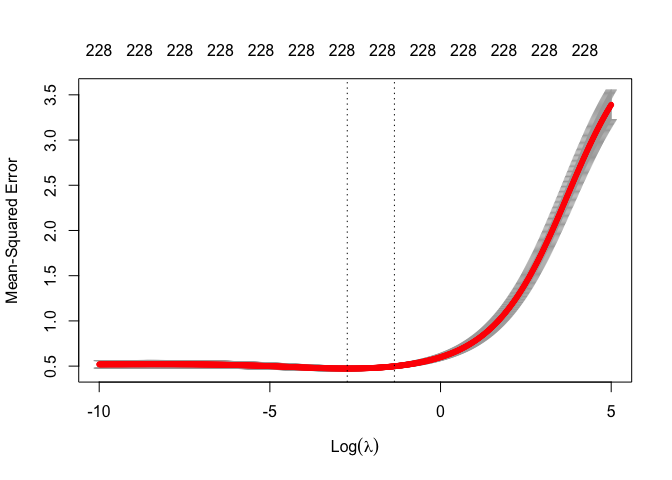
\includegraphics{hw1_files/figure-latex/unnamed-chunk-4-1.pdf}

\begin{Shaded}
\begin{Highlighting}[]
\NormalTok{cv.ridge}\OperatorTok{$}\NormalTok{lambda.min }\CommentTok{# min MSE}
\end{Highlighting}
\end{Shaded}

\begin{verbatim}
## [1] 0.06504131
\end{verbatim}

\begin{Shaded}
\begin{Highlighting}[]
\NormalTok{cv.ridge}\OperatorTok{$}\NormalTok{lambda}\FloatTok{.1}\NormalTok{se }\CommentTok{# 1se}
\end{Highlighting}
\end{Shaded}

\begin{verbatim}
## [1] 0.2588902
\end{verbatim}

\begin{Shaded}
\begin{Highlighting}[]
\NormalTok{ridge =}\StringTok{ }\KeywordTok{glmnet}\NormalTok{(xtrain, ytrain, }
               \DataTypeTok{standardize =} \OtherTok{TRUE}\NormalTok{,}
               \DataTypeTok{alpha =} \DecValTok{0}\NormalTok{,}
               \DataTypeTok{lambda =}\NormalTok{ cv.ridge}\OperatorTok{$}\NormalTok{lambda.min)}
\NormalTok{final_ridge =}\StringTok{ }\KeywordTok{predict}\NormalTok{(ridge, }\DataTypeTok{newx =} \KeywordTok{model.matrix}\NormalTok{(solubility }\OperatorTok{~}\NormalTok{., test)[,}\OperatorTok{-}\DecValTok{1}\NormalTok{], }\DataTypeTok{s =}\NormalTok{ cv.ridge}\OperatorTok{$}\NormalTok{lambda.min, }\DataTypeTok{type =} \StringTok{"response"}\NormalTok{)}
\NormalTok{mse_ridge =}\StringTok{ }\KeywordTok{mean}\NormalTok{(final_ridge }\OperatorTok{-}\StringTok{ }\NormalTok{test}\OperatorTok{$}\NormalTok{solubility)}\OperatorTok{^}\DecValTok{2}
\NormalTok{mse_ridge}
\end{Highlighting}
\end{Shaded}

\begin{verbatim}
## [1] 0.0004816
\end{verbatim}

\hypertarget{question-3-lasso-model}{%
\section{Question 3: Lasso Model}\label{question-3-lasso-model}}

\begin{Shaded}
\begin{Highlighting}[]
\KeywordTok{set.seed}\NormalTok{(}\DecValTok{1}\NormalTok{)}

\NormalTok{cv.lasso =}\StringTok{ }\KeywordTok{cv.glmnet}\NormalTok{(xtrain, ytrain, }
                     \DataTypeTok{type.measure =} \StringTok{"mse"}\NormalTok{,}
                     \DataTypeTok{alpha =} \DecValTok{1}\NormalTok{,}
                     \DataTypeTok{lambda =} \KeywordTok{exp}\NormalTok{(}\KeywordTok{seq}\NormalTok{(}\OperatorTok{-}\DecValTok{10}\NormalTok{, }\DecValTok{3}\NormalTok{, }\DataTypeTok{length =} \DecValTok{1000}\NormalTok{)))}
\KeywordTok{plot}\NormalTok{(cv.lasso)}
\end{Highlighting}
\end{Shaded}

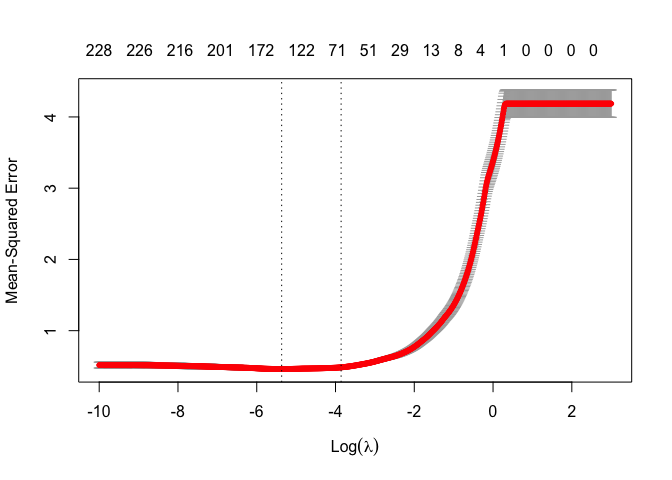
\includegraphics{hw1_files/figure-latex/unnamed-chunk-5-1.pdf}

\begin{Shaded}
\begin{Highlighting}[]
\NormalTok{cv.lasso}\OperatorTok{$}\NormalTok{lambda.min }\CommentTok{# min MSE}
\end{Highlighting}
\end{Shaded}

\begin{verbatim}
## [1] 0.0046664
\end{verbatim}

\begin{Shaded}
\begin{Highlighting}[]
\NormalTok{cv.lasso}\OperatorTok{$}\NormalTok{lambda}\FloatTok{.1}\NormalTok{se }\CommentTok{# 1se}
\end{Highlighting}
\end{Shaded}

\begin{verbatim}
## [1] 0.02111318
\end{verbatim}

\begin{Shaded}
\begin{Highlighting}[]
\NormalTok{lasso =}\StringTok{ }\KeywordTok{glmnet}\NormalTok{(xtrain, ytrain, }
               \DataTypeTok{standardize =} \OtherTok{TRUE}\NormalTok{,}
               \DataTypeTok{alpha =} \DecValTok{1}\NormalTok{,}
               \DataTypeTok{lambda =}\NormalTok{ cv.lasso}\OperatorTok{$}\NormalTok{lambda.min)}
\NormalTok{final_lasso =}\StringTok{ }\KeywordTok{predict}\NormalTok{(lasso, }\DataTypeTok{newx =} \KeywordTok{model.matrix}\NormalTok{(solubility }\OperatorTok{~}\NormalTok{., test)[,}\OperatorTok{-}\DecValTok{1}\NormalTok{], }\DataTypeTok{s =}\NormalTok{ cv.lasso}\OperatorTok{$}\NormalTok{lambda.min, }\DataTypeTok{type =} \StringTok{"response"}\NormalTok{)}
\NormalTok{mse_lasso =}\StringTok{ }\KeywordTok{mean}\NormalTok{(final_lasso }\OperatorTok{-}\StringTok{ }\NormalTok{test}\OperatorTok{$}\NormalTok{solubility)}\OperatorTok{^}\DecValTok{2}
\NormalTok{mse_lasso}
\end{Highlighting}
\end{Shaded}

\begin{verbatim}
## [1] 0.00109426
\end{verbatim}

\begin{Shaded}
\begin{Highlighting}[]
\KeywordTok{sum}\NormalTok{(final_lasso}\OperatorTok{!=}\DecValTok{0}\NormalTok{) }\CommentTok{# non-zero coefficients}
\end{Highlighting}
\end{Shaded}

\begin{verbatim}
## [1] 316
\end{verbatim}

\hypertarget{question-4-principle-component-regression-model}{%
\section{Question 4: Principle Component Regression
Model}\label{question-4-principle-component-regression-model}}

\end{document}
